\documentclass{article}%
\usepackage[T1]{fontenc}%
\usepackage[utf8]{inputenc}%
\usepackage{lmodern}%
\usepackage{textcomp}%
\usepackage{lastpage}%
\usepackage[head=40pt,margin=0.5in,bottom=0.6in]{geometry}%
\usepackage{graphicx}%
%
\title{\textbf{La Diáspora de Alicia}}%
\author{LINDA D'AMBROSIO}%
\date{04/03/2019}%
%
\begin{document}%
\normalsize%
\maketitle%
\textbf{URL: }%
http://www.eluniversal.com/el{-}universal/34522/la{-}diaspora{-}de{-}alicia\newline%
%
\textbf{Periodico: }%
EU, %
ID: %
34522, %
Seccion: %
el{-}universal\newline%
%
\textbf{Palabras Claves: }%
NO\_TIENE\newline%
%
\textbf{Derecho: }%
2.1%
, Otros Derechos: %
\newline%
%
\textbf{\textit{Es en febrero, sin embargo, cuando con más fuerza se deja sentir este carácter cultural en la urbe: se celebra ARCO, la feria de arte contemporáneo más importante en España}}%
\newline%
\newline%
%
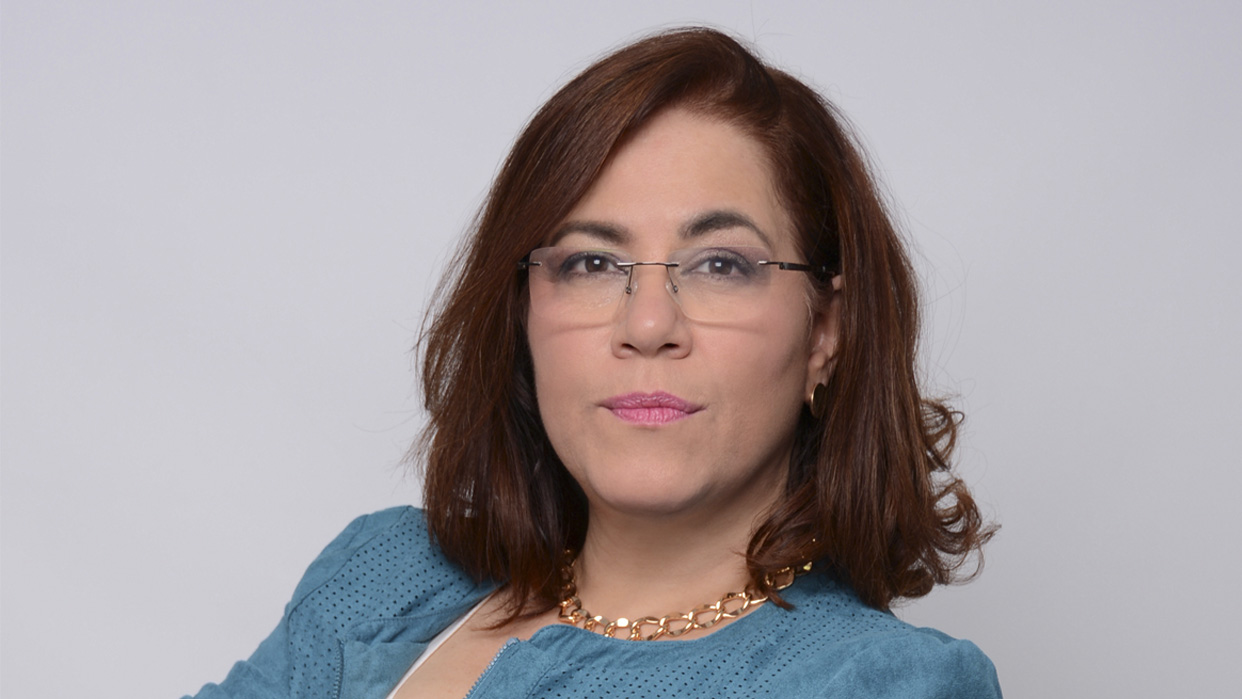
\includegraphics[width=300px]{EU_34522.jpg}%
\newline%
%
El arte es, sin duda alguna, una de las señas de identidad de Madrid. La ciudad no solo alberga instituciones como el Museo del Prado o el Thyssen Bormenisza, sino que en ella suelen tener lugar extraordinarias exposiciones.%
\newline%
%
Es en febrero, sin embargo, cuando con más fuerza se deja sentir este carácter cultural en la urbe: se celebra ARCO, la feria de arte contemporáneo más importante en España y una de las más destacadas de Europa.%
\newline%
%
En esta oportunidad 203 galerías de 30 países han convertido Madrid en la capital de la plástica y el coleccionismo. Pero es que simultáneamente se desarrolla otra serie de eventos que concitan la atención de los aficionados al arte: Urvanity, Drawing Room Madrid, Hybrid Art Fair, Generación2019, Producto Fresco, Ctrl Art Sup y la Feria SAM son algunas de las ferias que tienen lugar paralelamente en los más importantes centros culturales.%
\newline%
%
La ciudad respira arte. Nos encaminamos hacia la plaza de Callao, en la que convergen la Gran Vía y la calle Preciados, que desemboca en la archiconocida Puerta del Sol. Allí hay estructuras dispuestas para que se hagan demostraciones de Grafiti. De repente, al dar la vuelta a un módulo en que varios artistas están pintando murales, me da un vuelco el corazón y pierdo el aliento, como si me hubieran dado un puñetazo en el abdomen. En el suelo se despliega un círculo tricolor en que reconozco sin duda la bandera de Venezuela.%
\newline%
%
Alicia León Löbig desarrolla, a través de un collage de fotografías coloreadas, su personal experiencia de la diáspora gracias a una invitación de Fangisnow.%
\newline%
%
El amarillo, que alude a la riqueza, comprende las imágenes de un pasado feliz en el que hizo acopio de experiencias y recuerdos. El azul, sigue siendo el mar, ese mar que ella considera sinónimo de sanación y de limpieza, y que no se cansa de representar en sus obras… Las bellas playas venezolanas. Y el rojo es la sangre derramada, la propia sangre herida desde que su padre desapareciera de su finca en El Consejo, Estado Aragua. Superpuesta, se encuentra su fotografía, así como la copia de la denuncia de la desaparición.%
\newline%
%
Sobre el campo azul, siete aviones blancos de papel sustituyen las siete estrellas. La connotación es obvia.%
\newline%
%
Alicia llegó con su esposo y sus tres hijos en noviembre. Egresó con honores de la UCLA tras cursar la carrera de Bellas Artes. Ahora, se cose a la sudadera negra el retrato de su padre y su esposa, y un pequeño retazo de papel que inquiere: “¿Dónde están?”%
\newline%
%
Hace veinte años, cuando vine a vivir aquí, me inundaba una mezcla de orgullo y alegría cuando me topaba con algo que me vinculaba a mi tierra. Hoy son apenas señales de un mismo y único drama.%
\newline%
%
Otra vez. Otra historia. Otro venezolano fuera de su tierra. Así como demandaba Arquímedes “dadme un punto de apoyo y levantaré el mundo”, parece que los venezolanos dijeran “dadme una tribuna y gritaré esta tragedia”. No se puede explicar. Hay que haberlo vivido. No es la nostalgia por el hogar distante: es el dolor de la propia madre lacerada.%
\newline%
%
Sobre la alfombra de papel kraft en la que con pericia y una evidente economía de recursos Alicia cuenta visualmente su historia, firma y coloca el nombre de la obra: Memoria de mi diáspora.%
\newline%
%
Rematan la instalación, en la que también está presente su maleta, dos cuadernos.  Hay letreros que invitan a narrar algún recuerdo significativo en el de la  izquierda, y a expresar algún deseo, en  el de la derecha.%
\newline%
%
Me pongo de rodillas y empuño el bolígrafo. Sin que me tiemble el pulso, con el corazón y la mano en sintonía, escribo en el de los deseos una sola palabra:%
\newline%
%
¡Volver!%
\newline%
%
linda.dambrosiom@gmail.com%
\newline%
%
\end{document}